\documentclass[10pt]{article}
\usepackage{amsmath}
\usepackage[russian]{babel}
\usepackage{indentfirst}
\usepackage{amssymb}
\usepackage{amsfonts}
\usepackage{amsthm}
\usepackage[T2A]{fontenc}
\usepackage[utf8]{inputenc}
\usepackage{graphicx}
\usepackage{epigraph}
\usepackage{xcolor}
\usepackage{verbatim}
\usepackage{gensymb}
\usepackage{graphicx}
\usepackage[utf8]{inputenc}
\usepackage{lipsum}
\setlength{\parindent}{5ex}
\setlength{\parskip}{1em}
\graphicspath{}
\DeclareGraphicsExtensions{.pdf,.png,.jpg}
\usepackage{float}%"Плавающие" картинки
\usepackage{wrapfig}%Обтекание фигур (таблиц, картинок и прочего)
    

\begin{document}

\begin{center}
\begin{large}
\textbf{Условие домашнего задания №1}\\
Домашнее задание №1\\
по курсу "Численные методы" (СМ7, 3-й семестр, Осень\_2020)\\
\end{large}
\end{center}

Для заданной целевой функции на заданном отрезке (см. конец документа)найти:
\begin{enumerate}
\item Точку минимума (или в некоторых вариантах максимума).
\item Минимальное (максимальное) значение целевой функции.
Решить задачу тремя методами:
\begin{enumerate}
\item методом дихотомии;
\item методом золотого сечения;
\item методом квадратичной аппроксимации.
\end{enumerate}
\end{enumerate}
При поиске точки минимума рассмотреть для каждого метода три варианта с различными
значениями параметра точности поиска $\varepsilon =0,01; \varepsilon=0,00001$ и $\varepsilon=10^{-17}$. Для каждого варианта
вывести данные о количестве итераций и количестве вычисленных значений целевой функции (лучше в виде сводной таблицы) и построить графики изменения интервалов неопределенности.\\
\textbf{Объяснить полученные результаты. Работа должна заканчиваться выводами.}\\
Требования к выполнению, оформлению и сдачи домашнего задания.
\begin{enumerate}
\item Для выполнения домашнего задания использовать любые «математические пакеты» (MATLAB, SciLab, Octave, WolframMathematica, Mapleитд), а также любой язык программирования (Python, С/С++, JS… да хоть ассемблер). На худой конец ДЗ можно сделать даже в какой-нибудь электронной таблице (типа MicrosoftExcel).
\item Запрещено использовать только одну единственную программу: Mathcad.
\item Особо приветствуется в домашнем задании Julia $\ddot\smile$.
\item Запрещено использовать символьные вычисления и вычисления с произвольной точностью (например, VPA в MATLAB).
\item Работы без полностью заполненного титульного листа не принимаются.
\item Все страницы (кроме титульного листа) должны быть пронумерованы.
\item  Все рисунки и таблицы в тексте должны быть пронумерованы, подписаны и оформлены согласно ГОСТ 7.32-2017.
\item ГОСТа 7.32-2017 и здравого смысла придерживаться при оформлении всего домашнего задания: заголовки относятся к тексту, идущему после них; висячие строки и разрывы полей таблиц запрещены итд. Помните, что ваш текст прочитают не менее двух человек!
\textbf{\item  Сдача полностью одинаковых работ или работ с одинаковым кодом или выводами рассматривается как полное неуважение к Университету!}
\item Инициатива, расширение и углубление самого домашнего задания (например реализация связки МЗС+МКА, но не только) учитывается с повышенным коэффициентом.
\end{enumerate}

При сдачи работы в электронном виде в гуглоклассе использовать \textbf{только формат pdf}.
\newpage
Буду искать локальный максимум.\\
Отрезок - [-1, 0]\\
\[f(x) = \ln(2x^5-7x+\sqrt{11}) + \sh\left(\frac{-4x^2-4x+3-4\sqrt{2}}{3x^2+3x+3\sqrt{2}}\right) - 1.0\]
Задаем саму функцию:
\begin{verbatim}
def F(x): 
    return np.log(2 * x ** 5 - 7 * x + np.sqrt(11)) + np.sinh((-4 * x ** 2 - 4 * x 
    + 3 - 4 * np.sqrt(2)) / (3 * x ** 2 + 3 * x + 3 * np.sqrt(2))) - 1.0
\end{verbatim}
Также задам переменную max\_iters = 10000, которая будет сигнализировать о зацикливании.

\begin{figure}[h!]
\centering
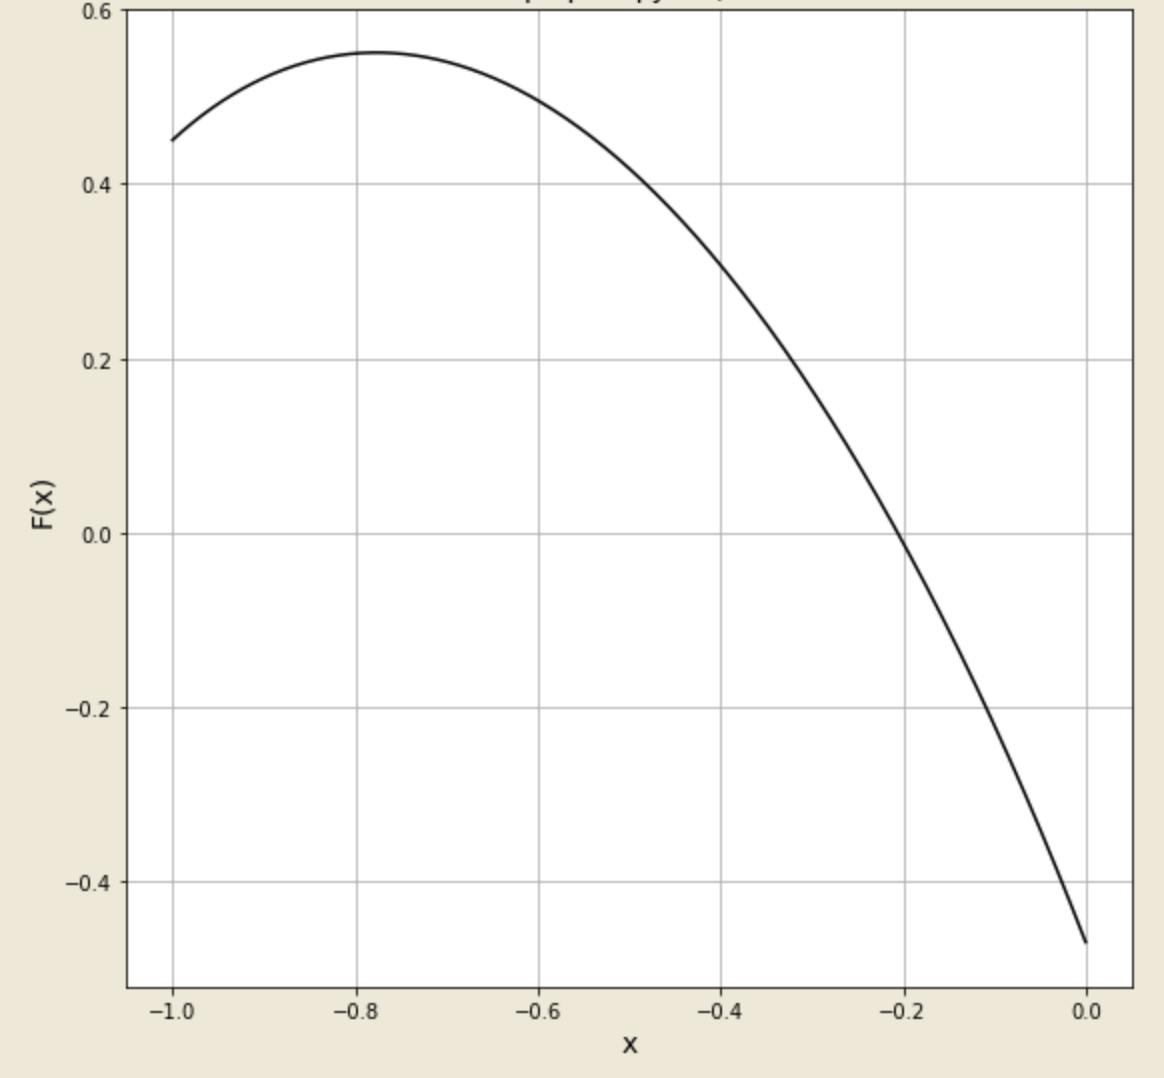
\includegraphics[width=0.8\linewidth]{f.png}
\caption{График функции}
\label{fig:image1}
\end{figure}
\newpage
\begin{enumerate}





\item
\begin{center}
\begin{large}
Метод  дихотомии.\\
\end{large}
\end{center}
Реализация на ЯП Python3:\\
\begin{verbatim}
def dichotomy(F, left, right, Eps, max_iters):
    counter = funcalls = 0  #Заведем перемнные для подсчета кол-ва 
    итераций и кол-ва вызовов ф-ции
    dotes, iters = [], [] # Инициализируем массив границ промежутка и итераций
    dotes.append([left, right])# Занесем в массив начальные конца отрезка
    iters.append(counter) # Занесем в массив начальную итерацию
    sigma = Eps / 2 # sigma - константая различимость
    while abs(right - left) > Eps and counter <= max_iters:
     #|right - left| < Eps - условие выхода
        x1 = (left + right - sigma)/2
         # Возьмем левый конец чуть левее середины отрезка
        x2 = (left + right + sigma)/2
         # Возьмем правый конец чуть правее середины отрезка
        if F(x1) * F(x2) > 0:
            left = x1
        else:
            right = x2
        dotes.append([left, right]) # Добавим новые концы отрезка
        counter += 1
        iters.append(counter) # Добавим следующую итерацию
        funcalls += 2
         # Т.к. в конструкци if-else мы вызываем ф-цию дважды, прибавляем 2
    return [(left + right) / 2, counter, funcalls, dotes, iters]
\end{verbatim}
\newpage
\begin{center}
Интервалы неопределенности для метода дихотомии.
\end{center}


\begin{table}[H]
\caption{Результаты метода дихотомии при $\varepsilon$ = 0.01}
\begin{center}
\begin{tabular}{|l|l|l|l|l|l|}
\hline
№ & X\_max    & F(X\_max) & Num of iters & Num of func calls & Eps  \\
\hline
    0  & -0.78  &    0.55 &               7 &                   14 &
0.01 \\
\hline
\end{tabular}
\end{center}
\end{table}

\begin{figure}[H]
\centering
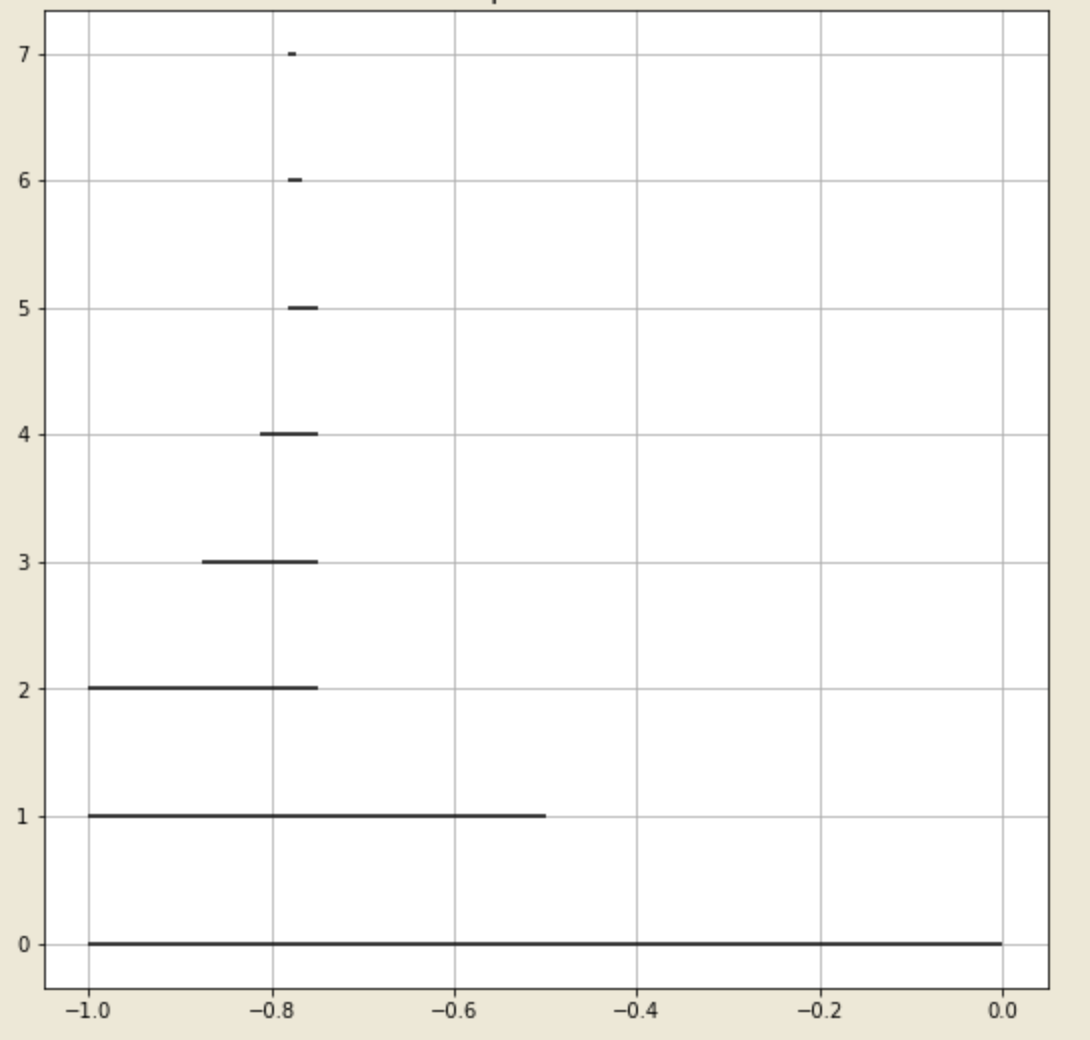
\includegraphics[width=0.8\linewidth]{1.png}
\caption{График изменения интервала неопределенности, $\varepsilon$ = 0.01}
\label{fig:image1}
\end{figure}
\newpage


\begin{table}[H]
\caption{Результаты метода дихотомии при $\varepsilon = 10^{-5}$}
\begin{center}
\begin{tabular}{|l|l|l|l|l|l|}
\hline
№ & X\_max    & F(X\_max) & Num of iters & Num of func calls & Eps  \\
\hline
     1  & -0.77665 &   0.55052 &              17 &                   34 &
1e-05 \\
\hline
\end{tabular}
\end{center}
\end{table}

\begin{figure}[H]
\centering
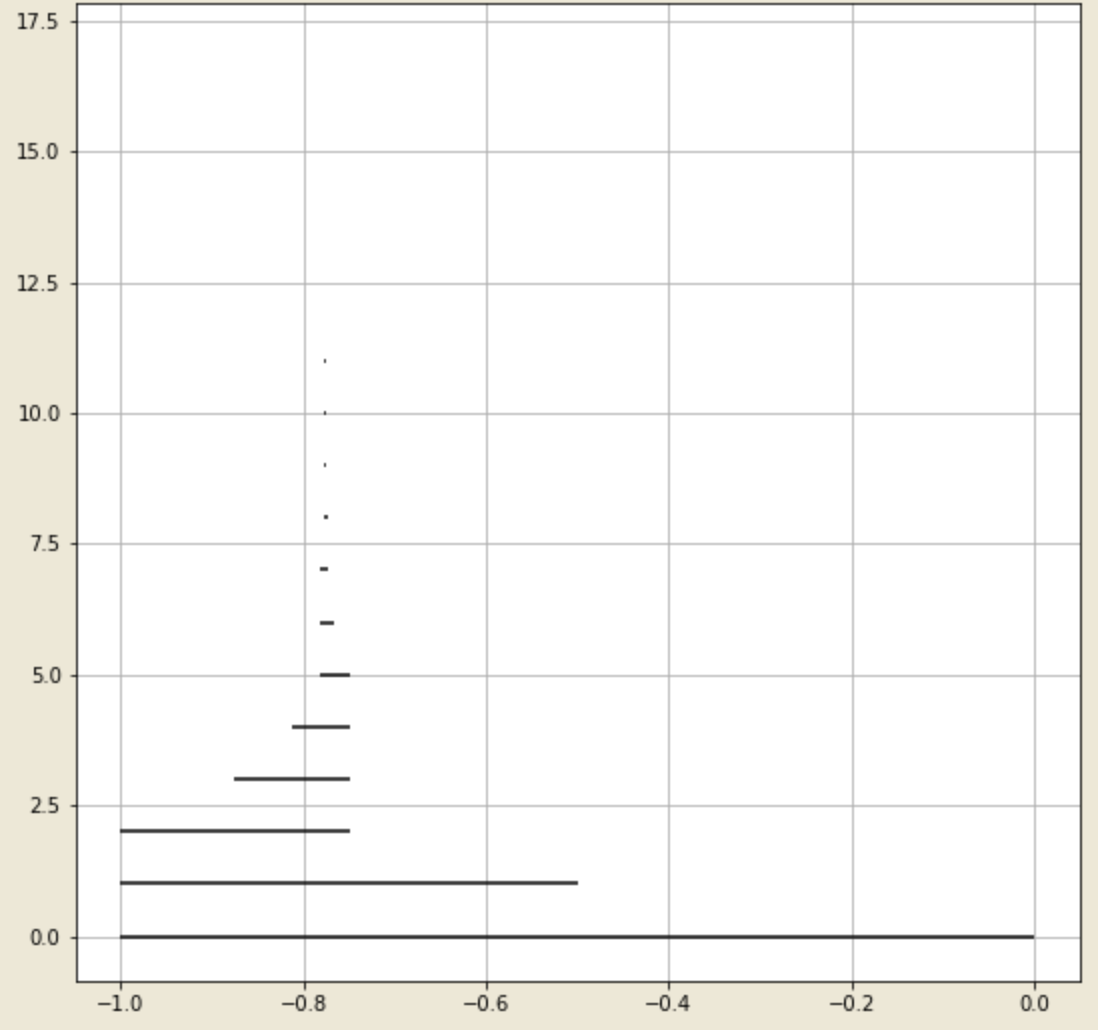
\includegraphics[width=0.8\linewidth]{2.png}
\caption{График изменения интервала неопределенности, $\varepsilon = 10^{-5}$}
\label{fig:image1}
\end{figure}
\newpage

\begin{table}[H]
\caption{Результаты метода дихотомии при $\varepsilon = 10^{-17}$}
\begin{center}
\begin{tabular}{|l|l|l|l|l|l|}
\hline
№ & X\_max    & F(X\_max) & Num of iters & Num of func calls & Eps  \\
\hline
    2 & -1.00000000000000000        &    0.45028971854510069  &              54 &                  108 &
1e-17 \\
\hline
\end{tabular}
\end{center}
\end{table}

\begin{figure}[H]
\centering
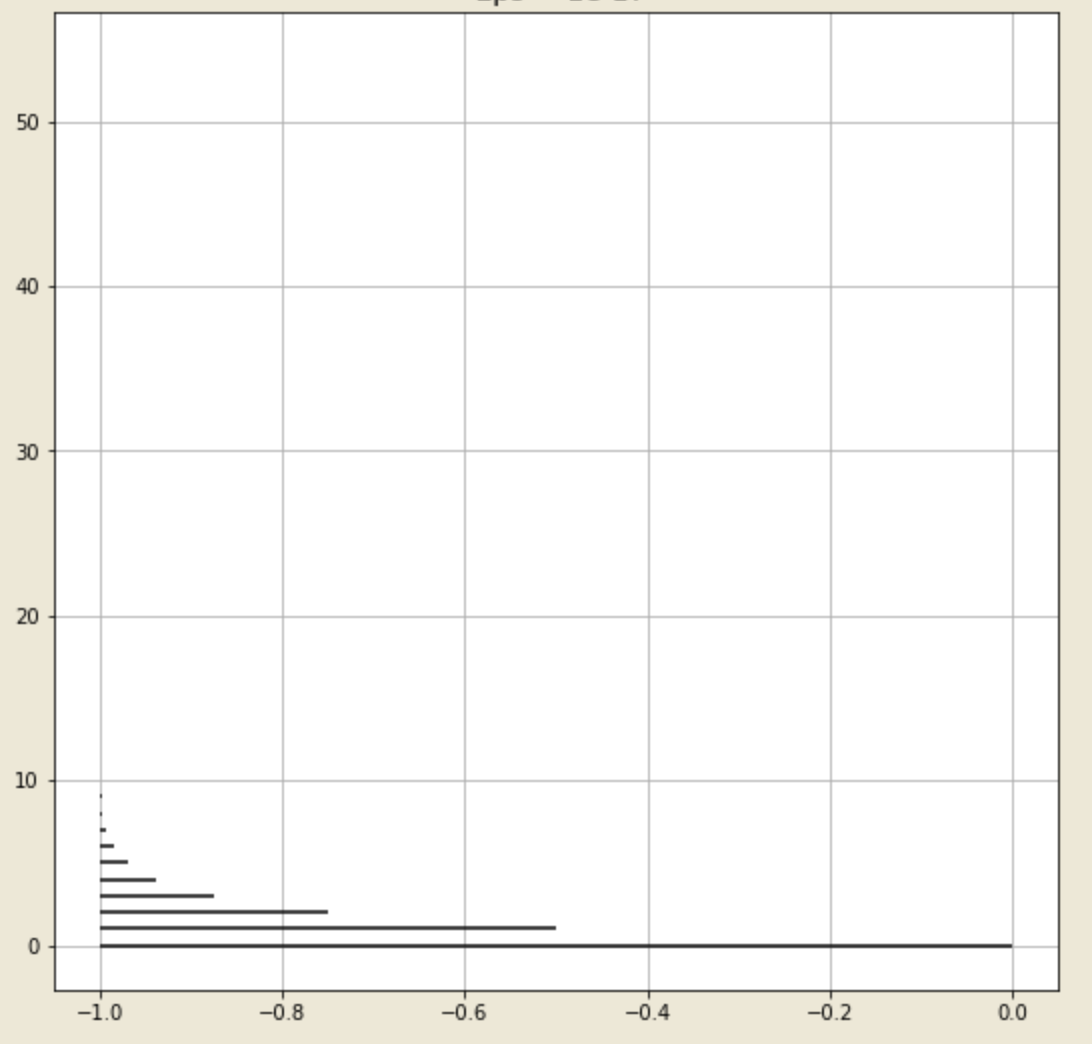
\includegraphics[width=0.8\linewidth]{3.png}
\caption{График изменения интервала неопределенности, $\varepsilon = 10^{-17}$}
\label{fig:image1}
\end{figure}
\newpage


\item
\begin{center}
\begin{large}
Метод золотого сечения.\\
\end{large}
\[\frac{b - a}{b - x_1} = \frac{b - a}{x_2 - a} = \Phi = \frac{1 + \sqrt{5}}{2}, \text{ где } \Phi - \text{пропорция золотого сечения.}\]
\[x_1 = b - \frac{b - a}{\Phi},\ x_2 = a + \frac{b - a}{\Phi}\]
\end{center}
\begin{center}
Реализация на ЯП Python3:\\
\end{center}
\begin{verbatim}
def GSC(F, left, right, Eps, max_iters):
    counter = funcalls = 0 
    # Заведем перемнные для подсчета кол-ва итераций и кол-ва вызовов ф-ции
    dotes, iters = [], [] # Инициализируем массив границ промежутка и итераций
    dotes.append([left, right]) # Занесем в массив начальные конца отрезка
    iters.append(counter) # Занесем в массив начальную итерацию
    x1 = right - (right - left) / ((1 + math.sqrt(5))/2)
     #точка x2 делит отрезок [x1, b] в отношении золотого сечения
    x2 = left + (right - left) / ((1 + math.sqrt(5))/2) 
    #точка x1 делит отрезок [a, x2] в отношении золотого сечения
    f1, f2 = F(x1), F(x2)
    funcalls += 2
    while True: # Реализуем цикл do-while
        if f1 >= f2: 
            right = x2
            x2 = x1
            f2 = f1
            x1 = right - (right - left) / ((1 + math.sqrt(5))/2)
            f1 = F(x1)
            funcalls += 1
        else:
            left = x1
            x1 = x2
            f1 = f2
            x2 = left + (right - left) / ((1 + math.sqrt(5))/2)
            f2 = F(x2)
            funcalls += 1
        dotes.append([left, right]) # Добавим новые концы отрезка
        counter += 1 # Увеличиваем итерацию
        iters.append(counter) # Добавим следующую итерацию
        if abs(right - left) < Eps or counter >= max_iters: 
            # |right - left| < Eps - условие выхода или же произойдет зацикл
            return [(right + left) / 2, counter, funcalls, dotes, iters]
\end{verbatim}
\newpage
\begin{center}
Интервалы неопределенности для метода золотого сечения.
\end{center}

\begin{table}[H]
\caption{Результаты метода золотого сечения при $\varepsilon = 0.01$}
\begin{center}
\begin{tabular}{|l|l|l|l|l|l|}
\hline
№ & X\_max    & F(X\_max) & Num of iters & Num of func calls & Eps  \\
\hline
    0 & -0.78  &   0.55 &               10 &                   12 &
0.01 \\
\hline
\end{tabular}
\end{center}
\end{table}

\begin{figure}[H]
\centering
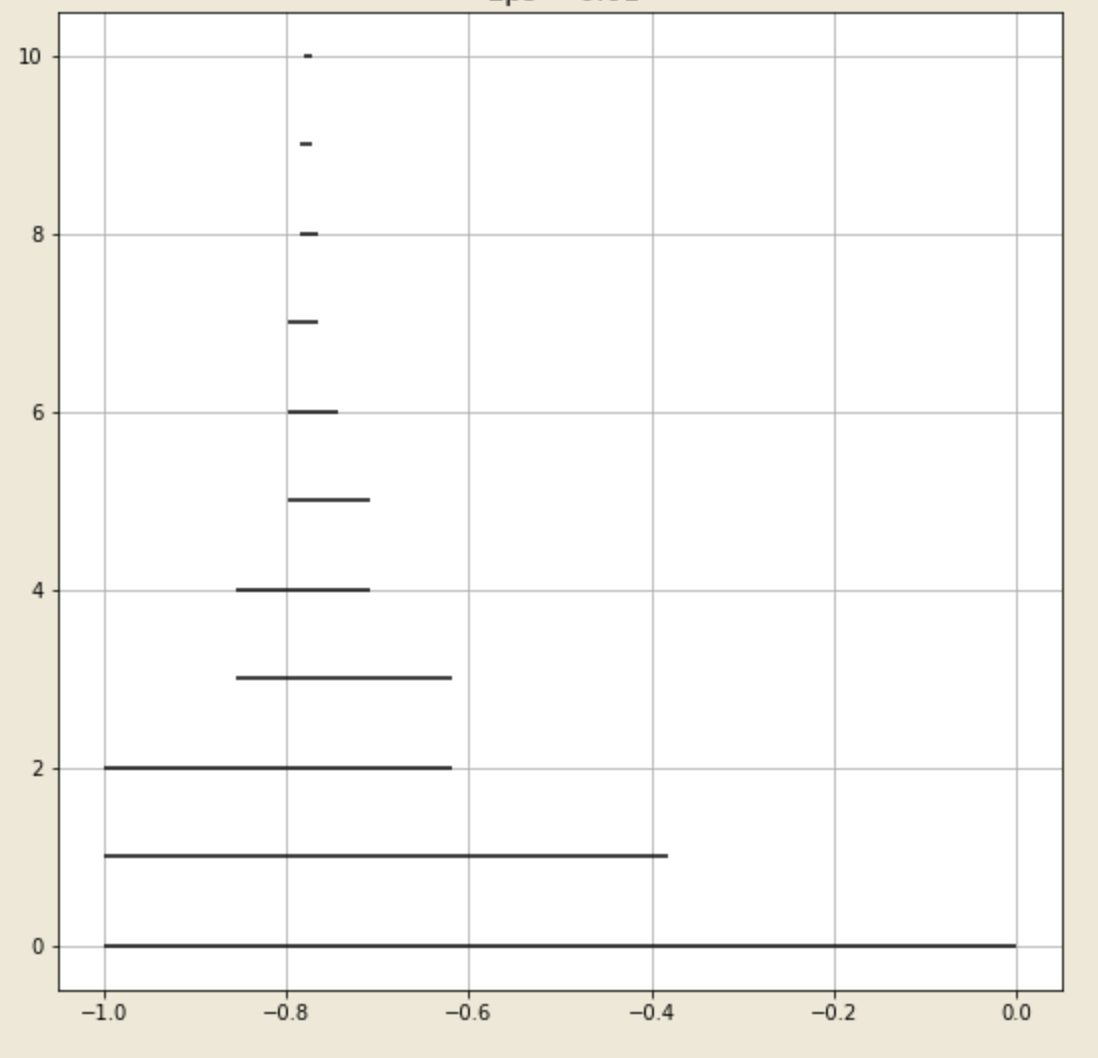
\includegraphics[width=0.8\linewidth]{4.png}
\caption{График изменения интервала неопределенности, $\varepsilon$ = 0.01}
\label{fig:image1}
\end{figure}
\newpage


\begin{table}[H]
\caption{Результаты метода золотого сечения при $\varepsilon = 10^{-5}$}
\begin{center}
\begin{tabular}{|l|l|l|l|l|l|}
\hline
№ & X\_max    & F(X\_max) & Num of iters & Num of func calls & Eps  \\
\hline
     1 & -0.77665 &   0.55052 &              24 &                   26 &
1e-05 \\
\hline
\end{tabular}
\end{center}
\end{table}

\begin{figure}[H]
\centering
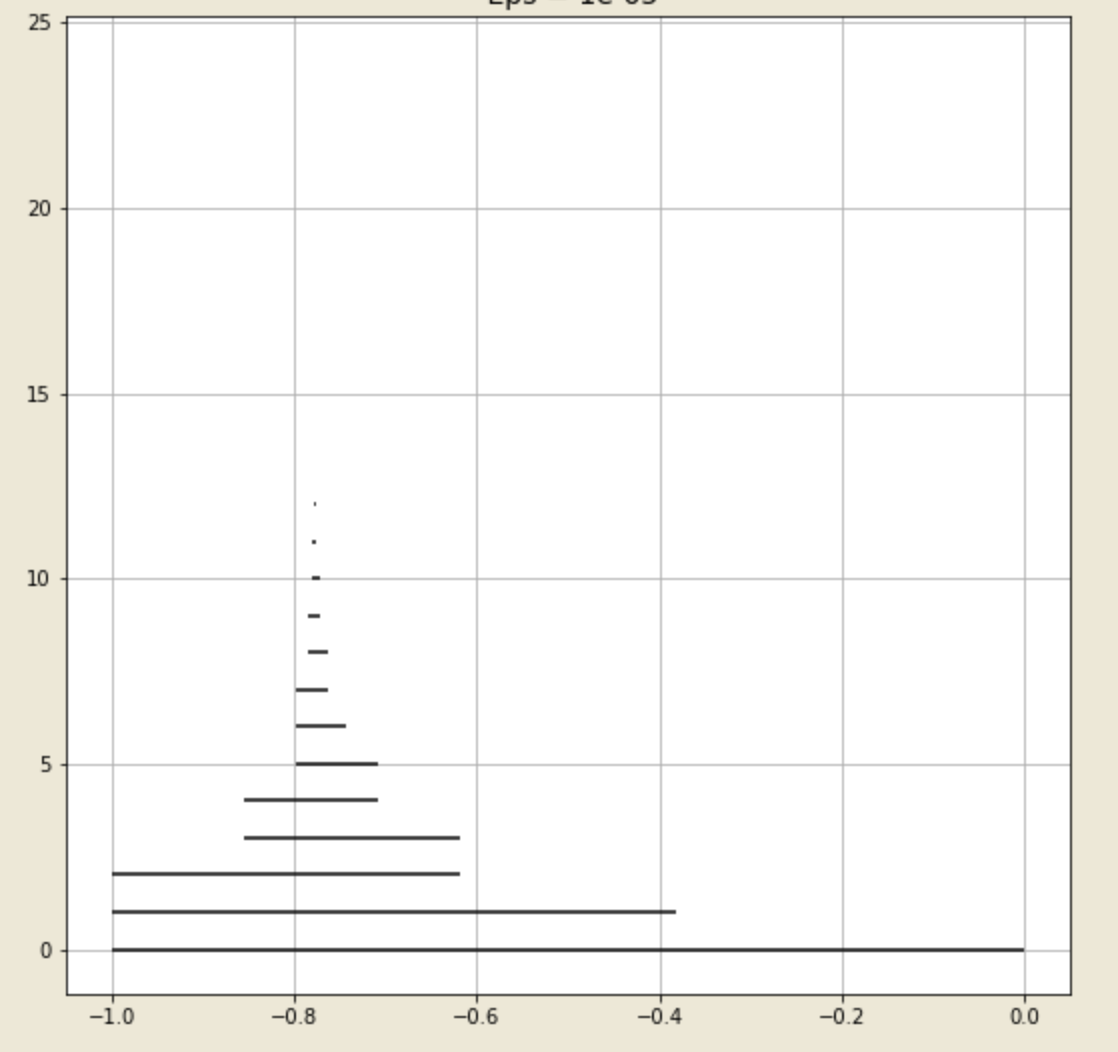
\includegraphics[width=0.8\linewidth]{5.png}
\caption{График изменения интервала неопределенности, $\varepsilon = 10^{-5}$}
\label{fig:image1}
\end{figure}
\newpage

\begin{table}[H]
\caption{Результаты метода золотого сечения при $\varepsilon = 10^{-17}$}
\begin{center}
\begin{tabular}{|l|l|l|l|l|l|}
\hline
№ & X\_max    & F(X\_max) & Num of iters & Num of func calls & Eps  \\
\hline
    2 & -0.77664964575113027          &    0.5505181509138641  &              100000 &                  100002 &
1e-17 \\
\hline
\end{tabular}
\end{center}
\end{table}

\begin{figure}[H]
\centering
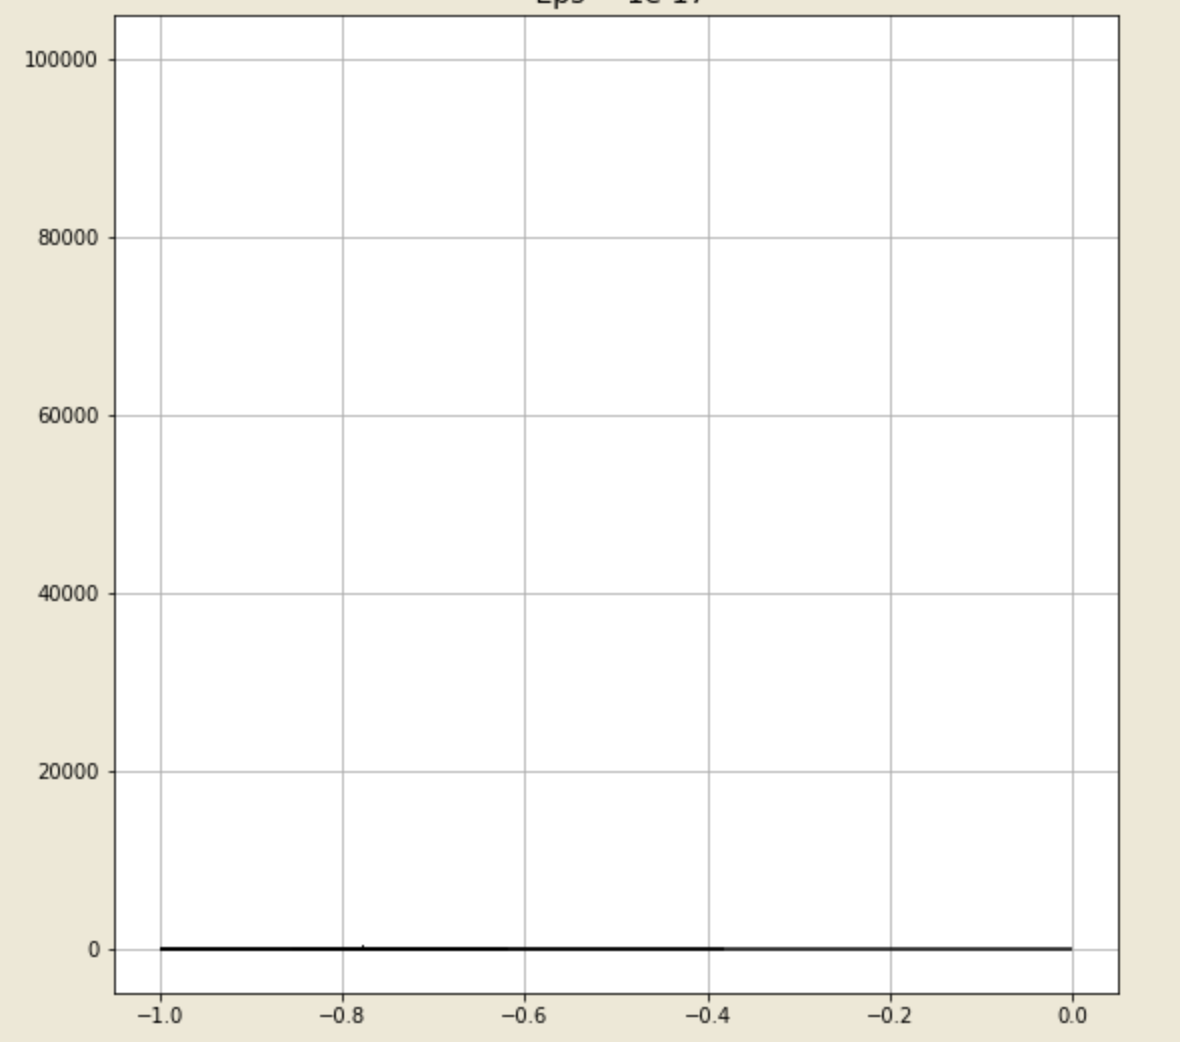
\includegraphics[width=0.8\linewidth]{6.png}
\caption{График изменения интервала неопределенности, $\varepsilon = 10^{-17}$}
\label{fig:image1}
\end{figure}
\newpage

\item
\begin{center}
\begin{large}
Метод квадратичной аппроксимации.\\
\end{large}
\end{center}
\begin{center}
Опишу формулы:\\
\end{center}
Начнем с того, что многочлен степени $n$ (т.е. $w_0 + w_1\cdot x = w_2\cdot x_2 + ... + w_n\cdot x_n)$ однозначно определяется любыми $n + 1$ точками, через которые он проходит. Таким образом, в методе квадратичной аппроксимации требуется задать 3 точки.\\
Квадратичная функция, которая должна совпасть со значениями f(x) в каждой из трех указанных точек:
\[q(x) = a_0 + a_1(x - x_1) + a_2(x-x_1)(x-x_2) .\]
\[f_1 = f(x_1) = q(x_1) = a_0,\Rightarrow a_0 = f_1.\]
\[f_2 = f(x_2) = q(x_2) = f_1 + a_1(x_2-x_1)\Rightarrow a_1 = \frac{f_2 - f_1}{x_2 - x_1}.\]
\[f_3 = f(x_3) = q(x_3) = f_1 = \frac{f_2 - f_1}{(x_2 - x_1)(x_3-x_1) + a_2(x_3-x_1)(x_3-x_2)}\Rightarrow\]
\[ a_2 = \frac{1}{x_3-x_2}\cdot \left(\frac{f_3-f_1}{x_3-x_1} - \frac{f_2-f_1}{x_2-x_1}\right)\]
По необходимому условию экстремума, найдем производную и с помощью нее выразим вершину параболы:
\[q'(x) = a_1 + a_2(x-x_2) + a_2(x-x_1) = 0\Rightarrow x = \frac{x_2 - x_1}{2} - \frac{a_1}{2a_2}.\]
\begin{center}
Реализация на ЯП Python3:\\
\end{center}
\begin{verbatim}

def powell(f, left, right, Eps, max_iters):
    h = 0.1 # Задаем шаг
    dotes, iters = [], [] # Инициализируем массив границ промежутка и итераций
    dotes.append([left, right]) # Занесем в массив начальные конца отрезка   
    funcalls, count = 0, 0
    iters.append(count) # Занесем в массив начальную итерацию
    
    
    x1, x2 = left, left +  h # Определим начальные точки
    i, j = 0, 0 
    # Индексация нам нужна, чтобы при выборе x_min мы 
    перестраивали массив выбирая "лучшую" точку и две другие с индексами i и j.
    x = [x1, x2]
    f1, f2 = f(x[0]), f(x[1])
    if f1 > f2:
        x3 = left + 2 * h
    else:
        x3 = left - h
    
    fx = [f1, f2, f(x3)]
    x.append(x3) # Занесем в массив x3, чтобы получить 3 начальные 
    точки x1, x2, x3.
    funcalls += 3
    
    dotes.append([x3, x1]) # Добавим новый интервал
    count += 1 # Добавим счетчик итераций
    iters.append(count) # Занесем в массив первую итерацию
    while True:
    		# Считаем коэффициенты многочлена:
        a1 = (fx[1] - fx[0]) / (x[1] - x[0])
        a2 = 1.0 / (x[2] - x[1]) * ((fx[2] - fx[0]) / (x[2]-x[0])-(fx[1]-fx[0]) /
         (x[1]-x[0]))
        x_max = (x[1] + x[0]) * 0.5 - a1 / (2 * a2)
        f_max = f(x_max)
        funcalls += 1
        # Здесь ищется x_max, который соответстует f_max= max(f1, max(f2, f3))
        if fx[0] >= fx[1]:
            if fx[0] >= fx[2]:
                i = 0
            else:
                i = 2
        else:
            if fx[1] >= fx[2]:
                i = 1
            else:
                i = 2
        count += 1
        iters.append(count)
        dotes.append([x[i], x_ max]]) 
        if ((abs((x_max - x[i]) / x_max) < Eps) and 
        (abs((f_max - fx[i])/f_max) < Eps)) or count >= max_iters:
            return [x_max, count, funcalls, dotes, iters]
        
        if fx[0] < fx[1]:
            if fx[0] <= fx[2]:
                j = 0
            else:
                j = 2
        else:
            if fx[1] <= fx[2]:
                j = 1
            else:
                j = 2
        
        if (f_max > fx[i]):
            x[j] = x_max
            fx[j] = f_max
        else:
            x[j] = 2 * x[i] - x_max
            fx[j] = F(x[j])
        
        
    return [x_max, count, funcalls, dotes, iters]
\end{verbatim}
\newpage
\begin{center}
Интервалы неопределенности для метода квадратичной аппроксимации.
\end{center}


\begin{table}[H]
\caption{Результаты метода квадратичной аппроксимации при $\varepsilon = 0.01$}
\begin{center}
\begin{tabular}{|l|l|l|l|l|l|}
\hline
№ & X\_max    & F(X\_max) & Num of iters & Num of func calls & Eps  \\
\hline
    0 & -0.78  &   0.55 &               3 &                   5 &
0.01 \\
\hline
\end{tabular}
\end{center}
\end{table}

\begin{figure}[H]
\centering
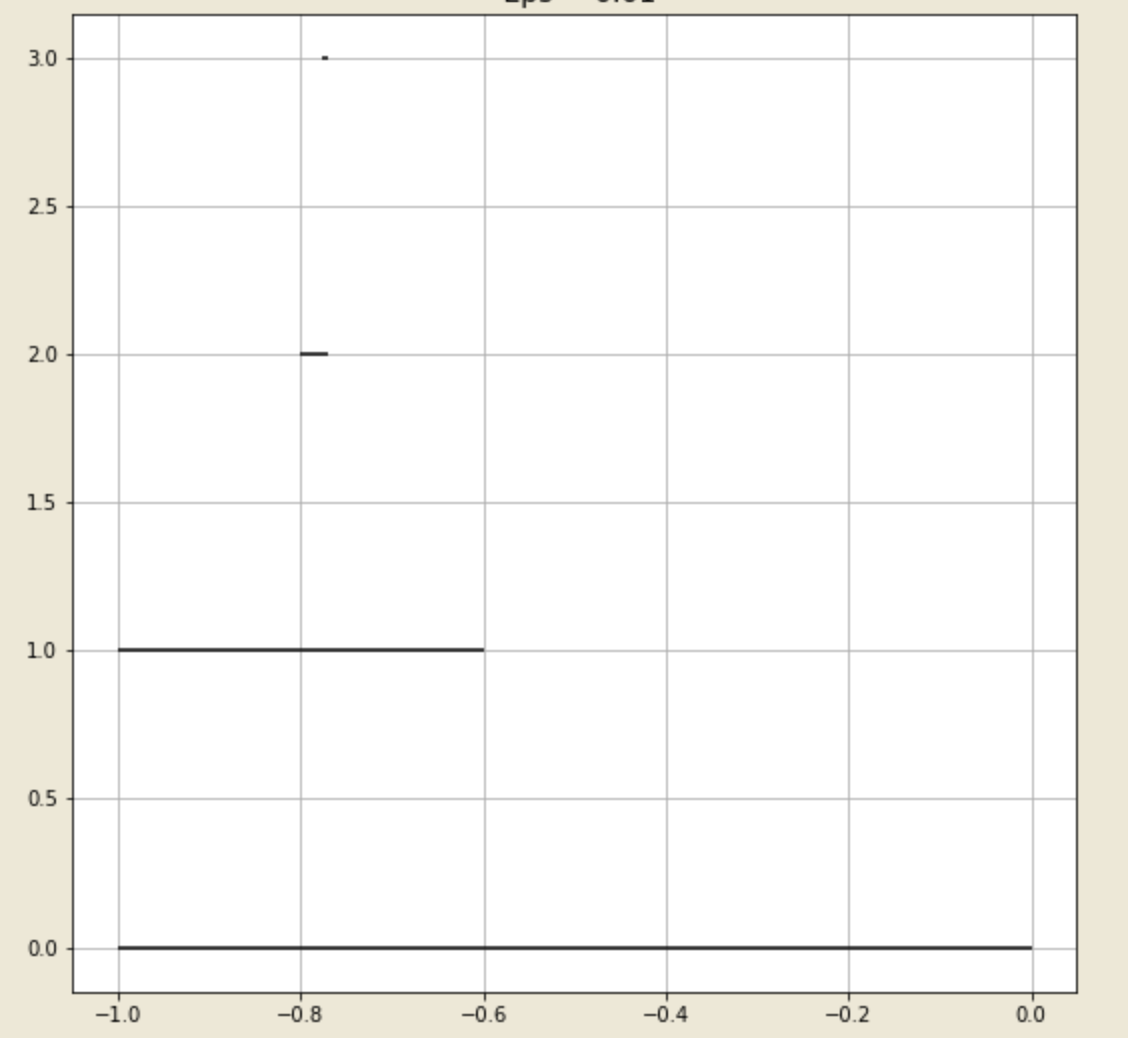
\includegraphics[width=0.8\linewidth]{7.png}
\caption{График изменения интервала неопределенности, $\varepsilon$ = 0.01}
\label{fig:image1}
\end{figure}
\newpage


\begin{table}[H]
\caption{Результаты метода квадратичной аппроксимации при $\varepsilon = 10^{-5}$}
\begin{center}
\begin{tabular}{|l|l|l|l|l|l|}
\hline
№ & X\_max    & F(X\_max) & Num of iters & Num of func calls & Eps  \\
\hline
     1 & -0.77658 &  0.55052 &              6 &                   8 &
1e-05 \\
\hline
\end{tabular}
\end{center}
\end{table}

\begin{figure}[H]
\centering
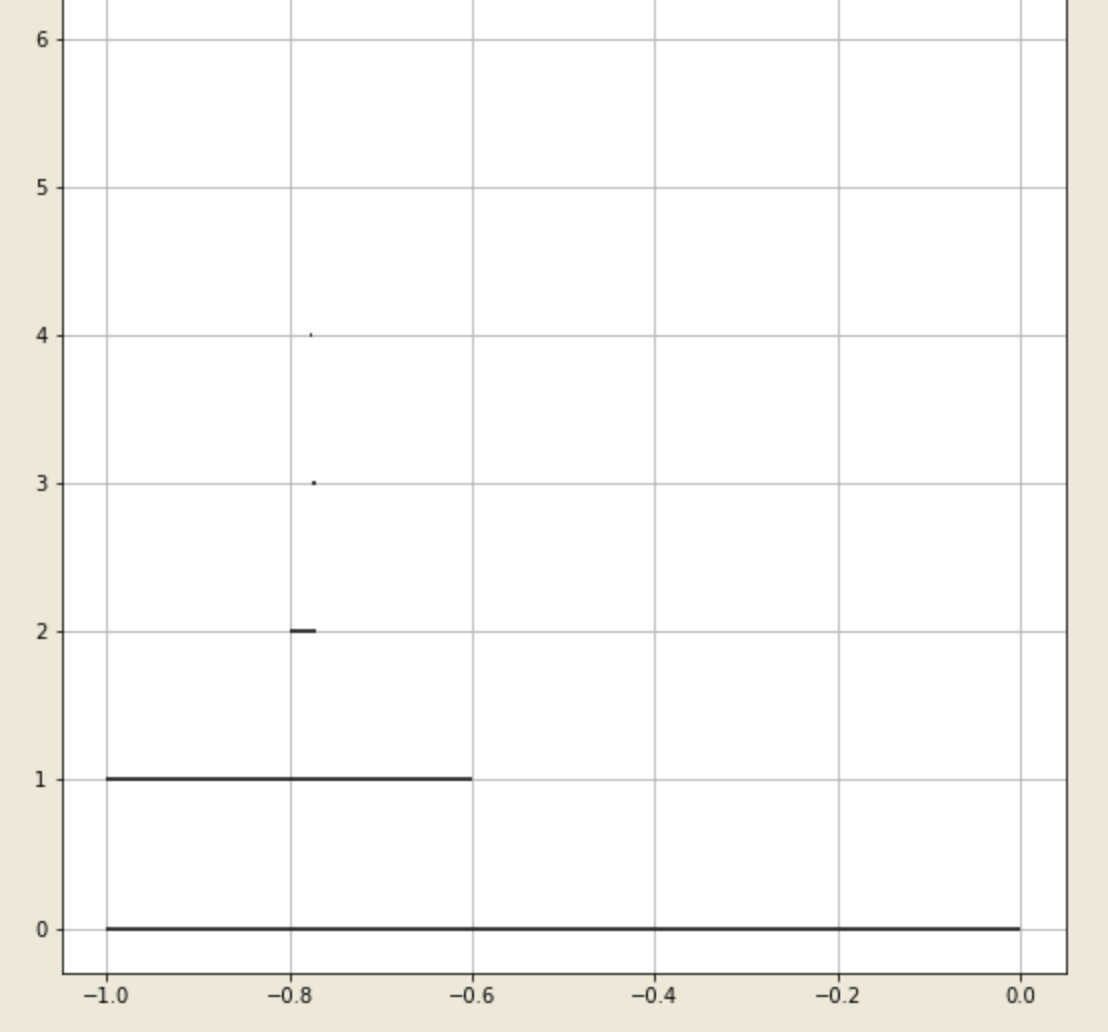
\includegraphics[width=0.8\linewidth]{8.png}
\caption{График изменения интервала неопределенности, $\varepsilon = 10^{-5}$}
\label{fig:image1}
\end{figure}
\newpage


\begin{table}[H]
\caption{Результаты метода квадратичной аппроксимации при $\varepsilon =10^{-17}$}
\begin{center}
\begin{tabular}{|l|l|l|l|l|l|}
\hline
№ & X\_max    & F(X\_max) & Num of iters & Num of func calls & Eps  \\
\hline
    2 & -0.77664965664046193          &    0.5505181509138641  &              100000 &                  100002 &
1e-17 \\
\hline
\end{tabular}
\end{center}
\end{table}

\begin{figure}[H]
\centering
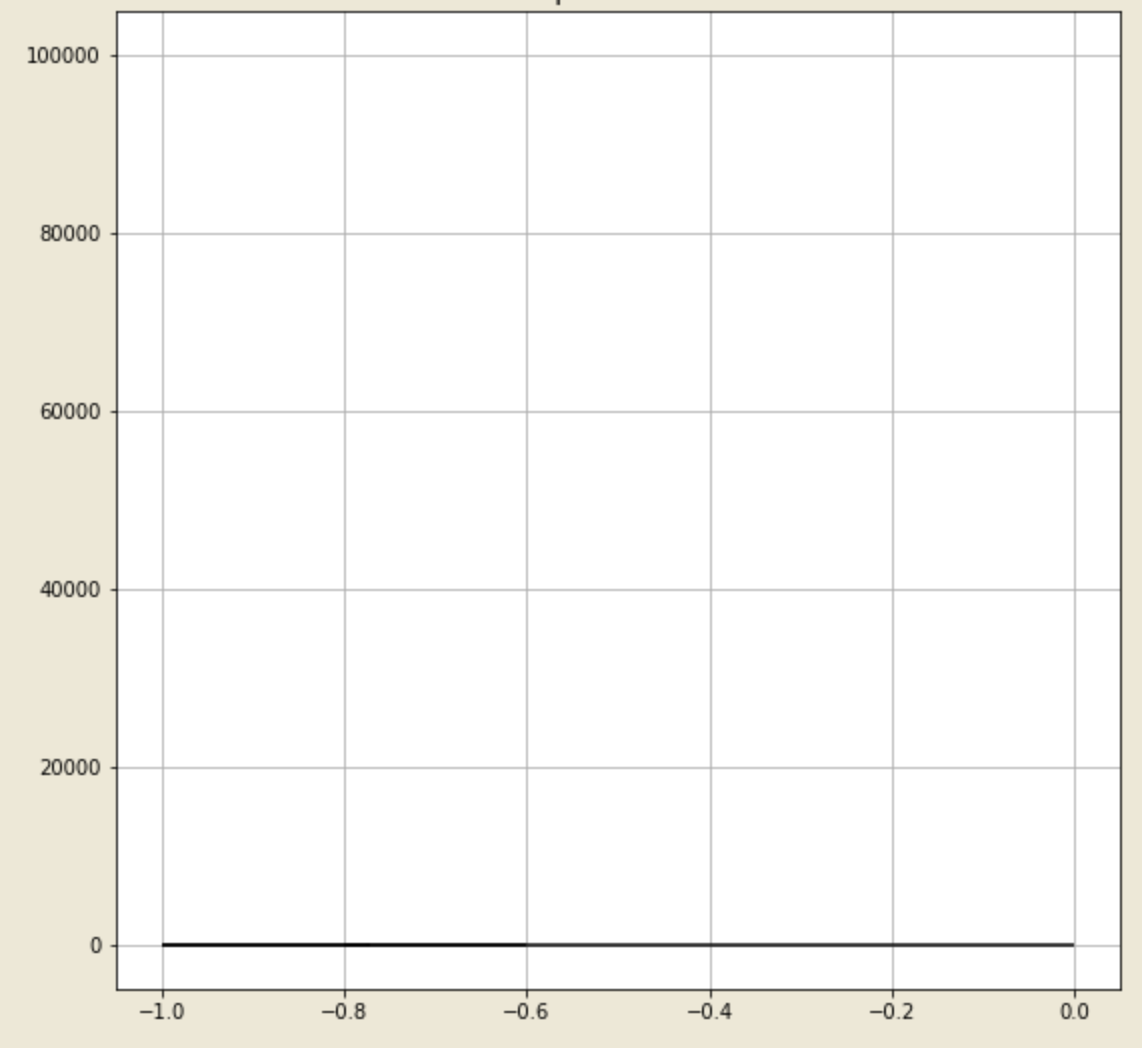
\includegraphics[width=0.8\linewidth]{9.png}
\caption{График изменения интервала неопределенности, $\varepsilon = 10^{-17}$}
\label{fig:image1}
\end{figure}


\end{enumerate}
\newpage
\begin{center}
\begin{large}
Выводы:\\
\end{large}
\end{center}
\begin{enumerate}
\item Метод дихотомии:
\begin{enumerate}
\item Сам метод прост, как в реализации, так и в действии;  
\item Так как функция будет рассматривать точки $x_1$ и $x_2$, вне зависимости от данных, алгоритм будет работать с любыми данными также, как и в в худшем. Т.е. мы будем рассматривать множество лишних данных;  
\item При увелечении количества итераций элементы дихотомического деления, будут более схожи между собой, т.е. $x_1$ и $x_2$ будут очень близки по значению, что затрудняет поиск локального экстремума; 
\item При уменьшении Eps, наш отрезок [left, right] может становиться большей длины, что повлияет на точность вычисления $x_{max}$.  
\end{enumerate}
\item Метод золотого сечения :
\begin{enumerate}
\item Аналогично, метод довольно таки прост;  
\item Eps начинает влиять на результат, лишь увеличивает при очень малых значениях(например, 1e-17);
\item При малых Eps происходит зацикливание, например, при Eps = $1e-17$, это происходит потому что при интервал неопределенности уже достигает точности в $1e-16$ и не может выйти из цикла, ибо не меньше $1e-17$, но и уменшиться не может, ибо он дошел до своего конечного ответа.
\item Алгоритм универсален, в плане поступающих данных. Т.е. поступят плохие данные - отработает плохо, иначе  - хорошо. Под словами 'хорошо' и 'плохо', я имею в виду, что может достигаться как нижняя, так и верхняя ассимптотическая граница алгоритма.
\end{enumerate}
\item Метод квадратичной аппроксимации:
\begin{enumerate}
\item Алгоритм средней сложности в реализцаии;  
\item Eps начинает влиять на результат, лишь увеличивает при очень малых значениях(например, 1e-17);
\item Алгоритм быстродейственный;
\item Зацикливание происходит при очень малой точности, например при Eps = $1e-17$, это происходит потому что при малых eps теряется точность чисел с плавающей точкой. Данное Eps будет превышать конечный интервал поиска, поэтому цикл не остановится. Hаш реузльтат точно еще меньше, чем шаг между ними, поэтому когда он находит новое значение он не может найти, потому что зацикливается около старого значения.
\item Алгоритм не справиться с линейными функциями, так как мы аппроксимируем функцию параболой, наша функция должна быть многочленом как минимум второй степени.
\end{enumerate}
\end{enumerate}
Из-за того что на больших отрезках метод квадратичной аппроксимации не очень точный, в голову приходит мысль оптимизации.\\
Если мы модифицируем алгоритм, т.е. при больших интервалах будем использовать метод золотого сечения, а при малых метод Пауэлла, мы получим самый оптимальный алгоритм из вышепредложенных.
\newpage
\begin{center}
\begin{large}
Источники
\end{large}
\end{center}
\begin{itemize}

\item Метод дихотомии\\
http://www.machinelearning.ru/wiki/index.php?title=Методы\_дихотомии
\item Метод золотого сечения\\
https://ru.wikipedia.org/wiki/Метод\_золотого\_сечения
\item Метод квадратичной аппроксимации\\
 http://knigechka.blogspot.com/2010/04/blog-post\_6723.html
\end{itemize}
\end{document}